% Para adicionar uma imagem ou incluir um arquivo .tex você precisa 
% adicionar \CWD
% caminho relativo (ao documento principal) do diretório.
% 
% Exemplo:
% \begin{figure}
%   \includegraphics{\CWD/imagens/exemplo.pdf}
% \end{figure}

We have to find the \textbf{densest} subgraph, but taking node weights into account.

Let's assume we have guess $G$ (real number) of the maximum score.
If we can determine if a subgraph $S \subseteq V$ exists with a score $> G$, we can binary search the answer.

We can model this comparison as a max-flow problem using the following graph: every edge and vertex of the original graph are represented with nodes as follows:

\begin{figure}[!tbh]
	\centering
	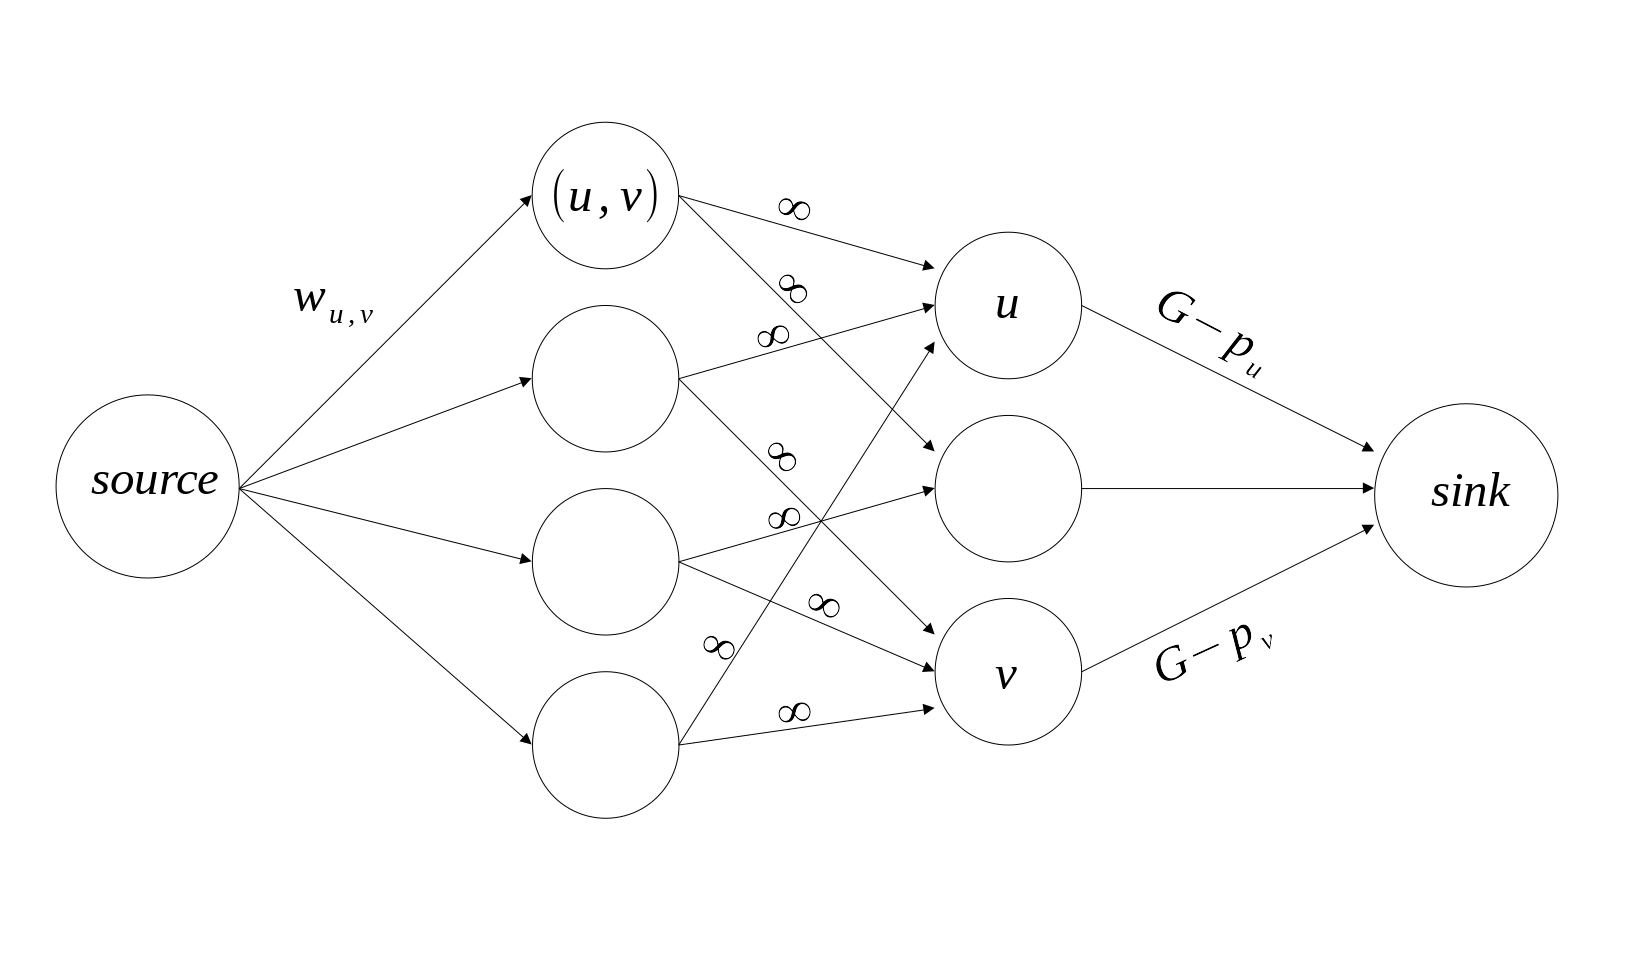
\includegraphics[width=0.5\linewidth]{\CWD/images/network.png}
\end{figure}

We can re-arrange the score function compared to our guess $G$ as follows, akin to the flow network:

\begin{equation*}
    \begin{split}
        \frac{\sum\limits_{u \in S} {p_u} + \sum\limits_{\substack{(u, v, w) \in E \\ u, v \in S}} {w_{u, v}}}{\lvert S \rvert} \quad & ? \quad G \\ \\
        \sum\limits_{\substack{(u, v, w) \in E \\ u, v \in S}} {w_{u, v}} \quad & ? \quad G \cdot {\lvert S \rvert} - \sum\limits_{u \in S} {p_u} \\ \\
        \sum\limits_{\substack{(u, v, w) \in E \\ u, v \in S}} {w_{u, v}} \quad & ? \quad \sum\limits_{u \in S} {G - p_u}
    \end{split}
\end{equation*}

The left side of the equation represent the edges within $S$, leaving the $source$. The right side represent the vertices of $S$ e.g. edges reaching the $sink$.

By running a max-flow algorithm in the described network for a guess $G$:
\begin{itemize}
    \item If the left side is $\le$ the right side of the equation, then all edges from the $source$ will be saturated, so the source-side of the cut will be just $\{source\}$. \\
    \item If the left side is $>$ the right side the equation, some edges won't be saturated; moreorver, the source-side of the cut will contain the nodes that represent $S$ in the riginal graph s.t. $score(S) > G$. \\
\end{itemize}

We can do a binary search for the maximum score, using any max-flow algorithm, keeping the source-side of the cut as the final answer.

Implemented with Dinic's max-flow algorithm, the worst case complexity is $\mathcal{O}((V + E)^3 \cdot \log X)$, but runs much faster in practice due to the shape of the graph. \\
There's also an alternative (smaller) construction for the flow graph that can achieve $\mathcal{O}(V^2 \cdot E \cdot \log X)$ when implementedd with Dinic's algorithm, but this is not required to get AC.
